\chapter{Fe-Pd and Fe-Ru Structures}
\label{chapter:appendix-fepd-feru-structures}


\section{Potential vs DFT}

\begin{figure}[htb]
\centering
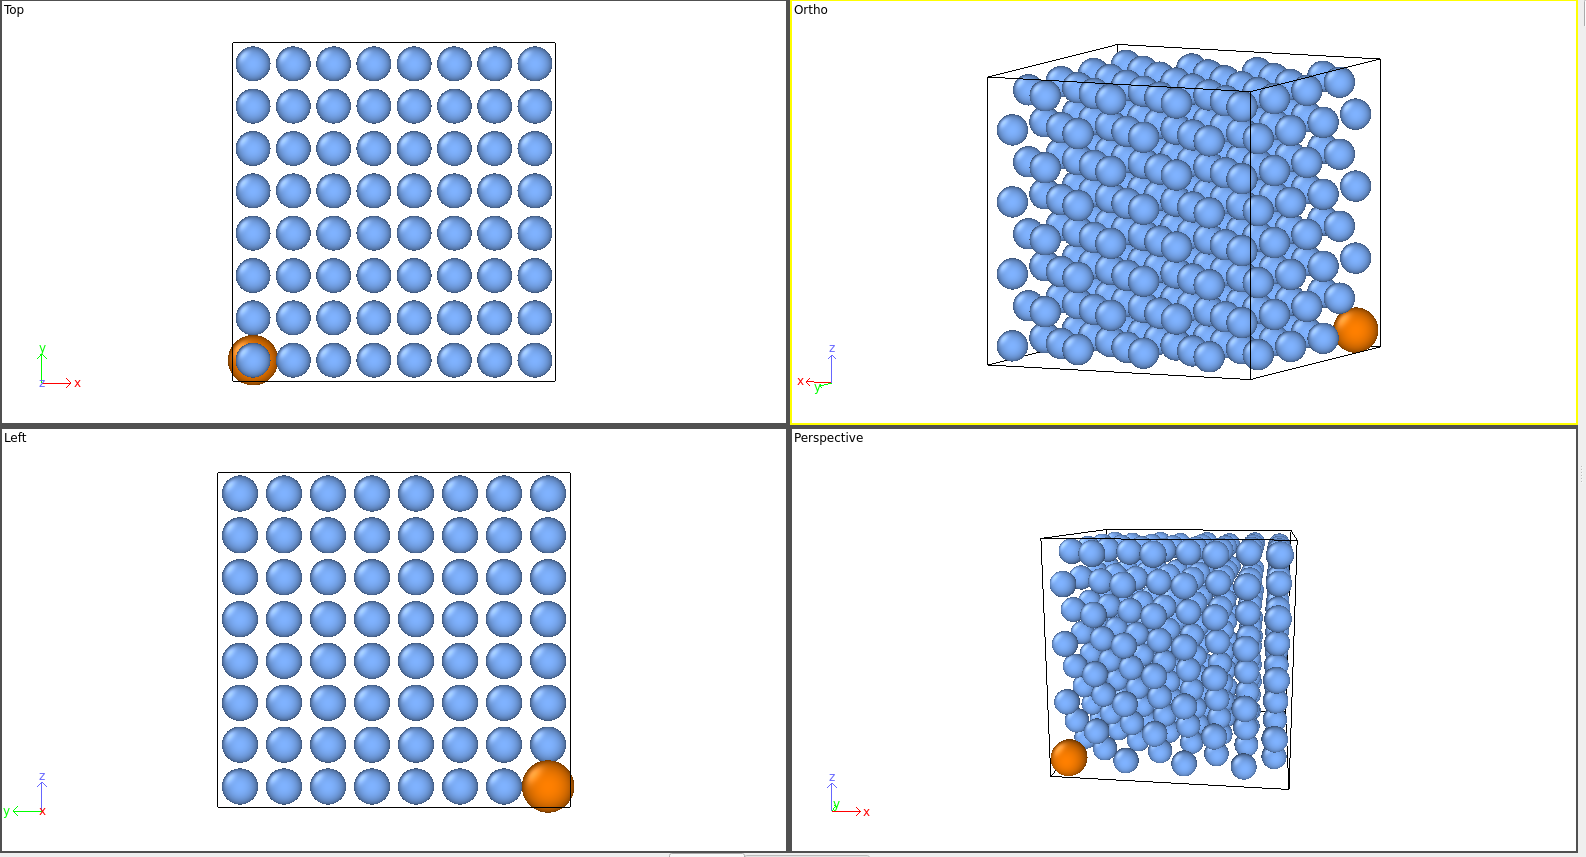
\includegraphics[width=.85\linewidth]{appendix/fepd_feru_configurations/fepd/fepd256_01r.png}  
\caption{FePd Structure 01}
\label{fig:fepd01}
\end{figure}

\begin{figure}[htb]
\centering
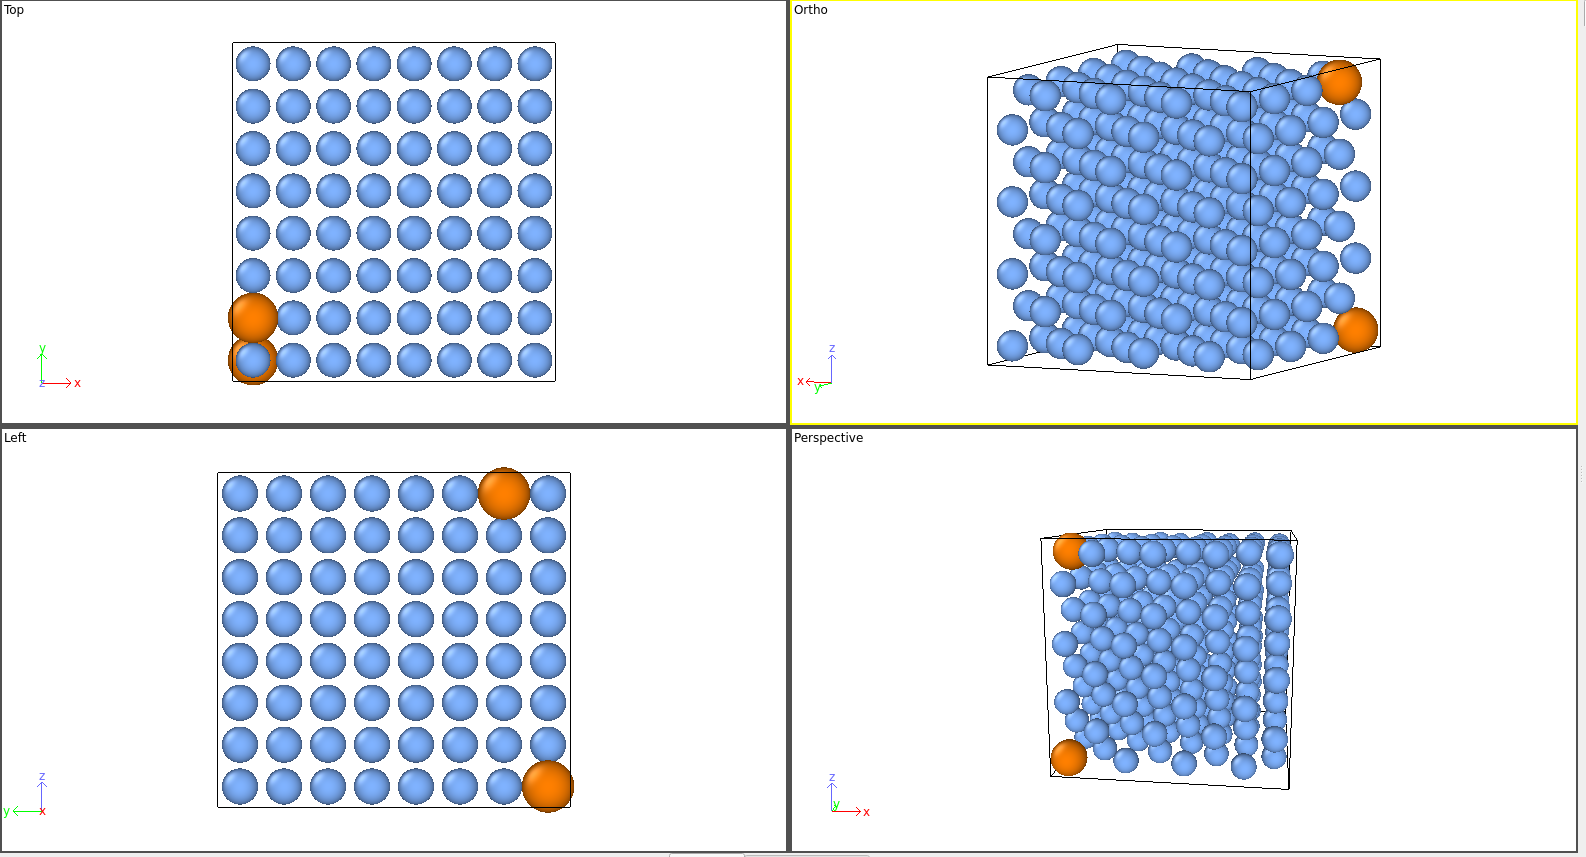
\includegraphics[width=.85\linewidth]{appendix/fepd_feru_configurations/fepd/fepd256_02r.png}  
\caption{FePd Structure 02}
\label{fig:fepd02}
\end{figure}

\begin{figure}[htb]
\centering
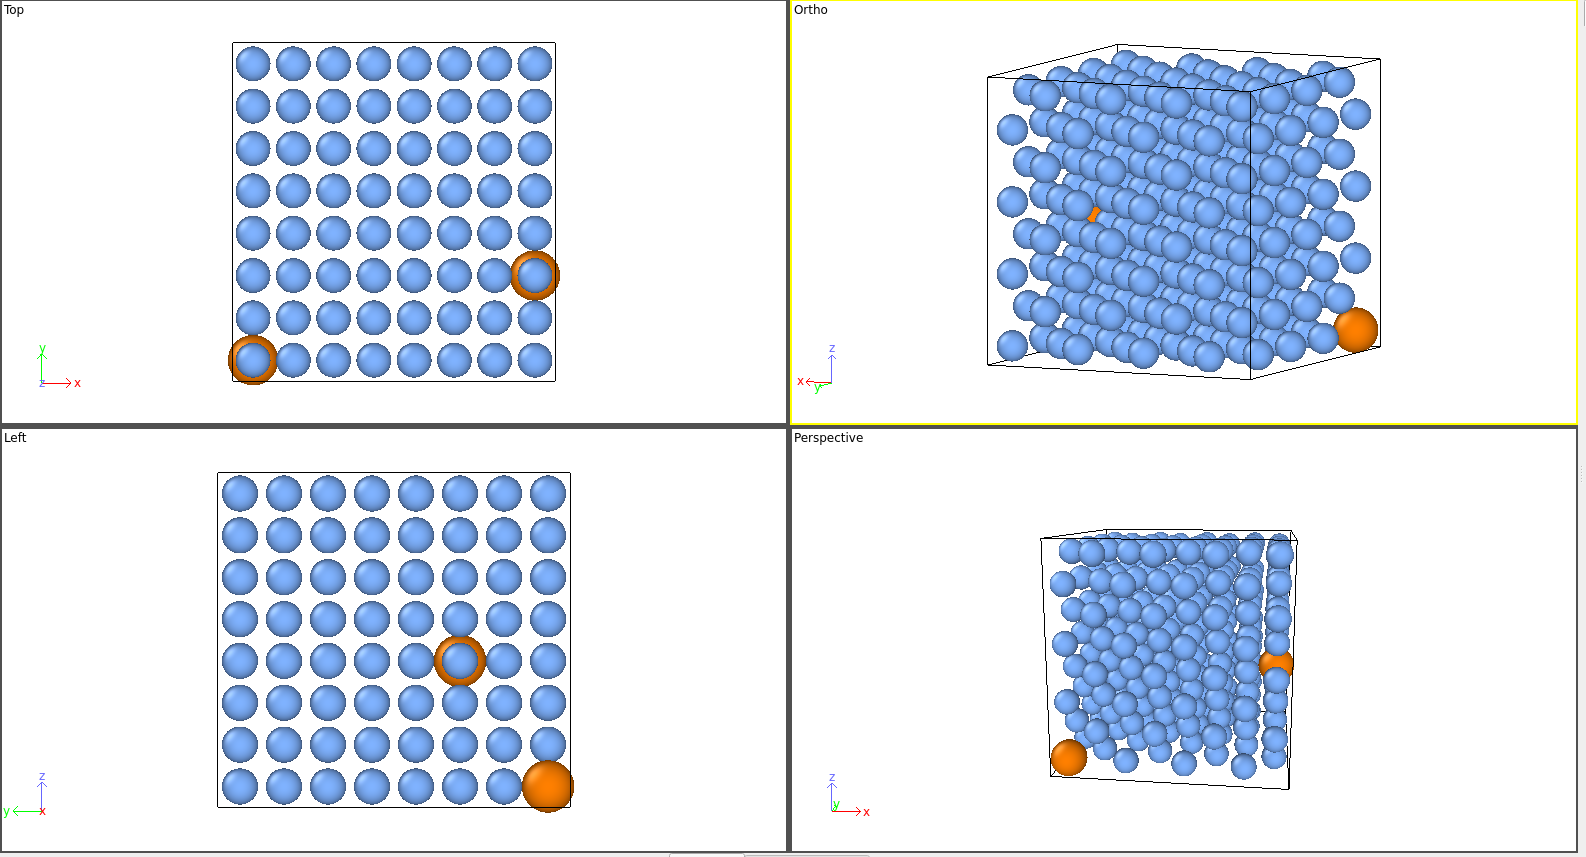
\includegraphics[width=.85\linewidth]{appendix/fepd_feru_configurations/fepd/fepd256_03r.png}   
\caption{FePd Structure 03}
\label{fig:fepd03}
\end{figure}

\begin{figure}[htb]
\centering
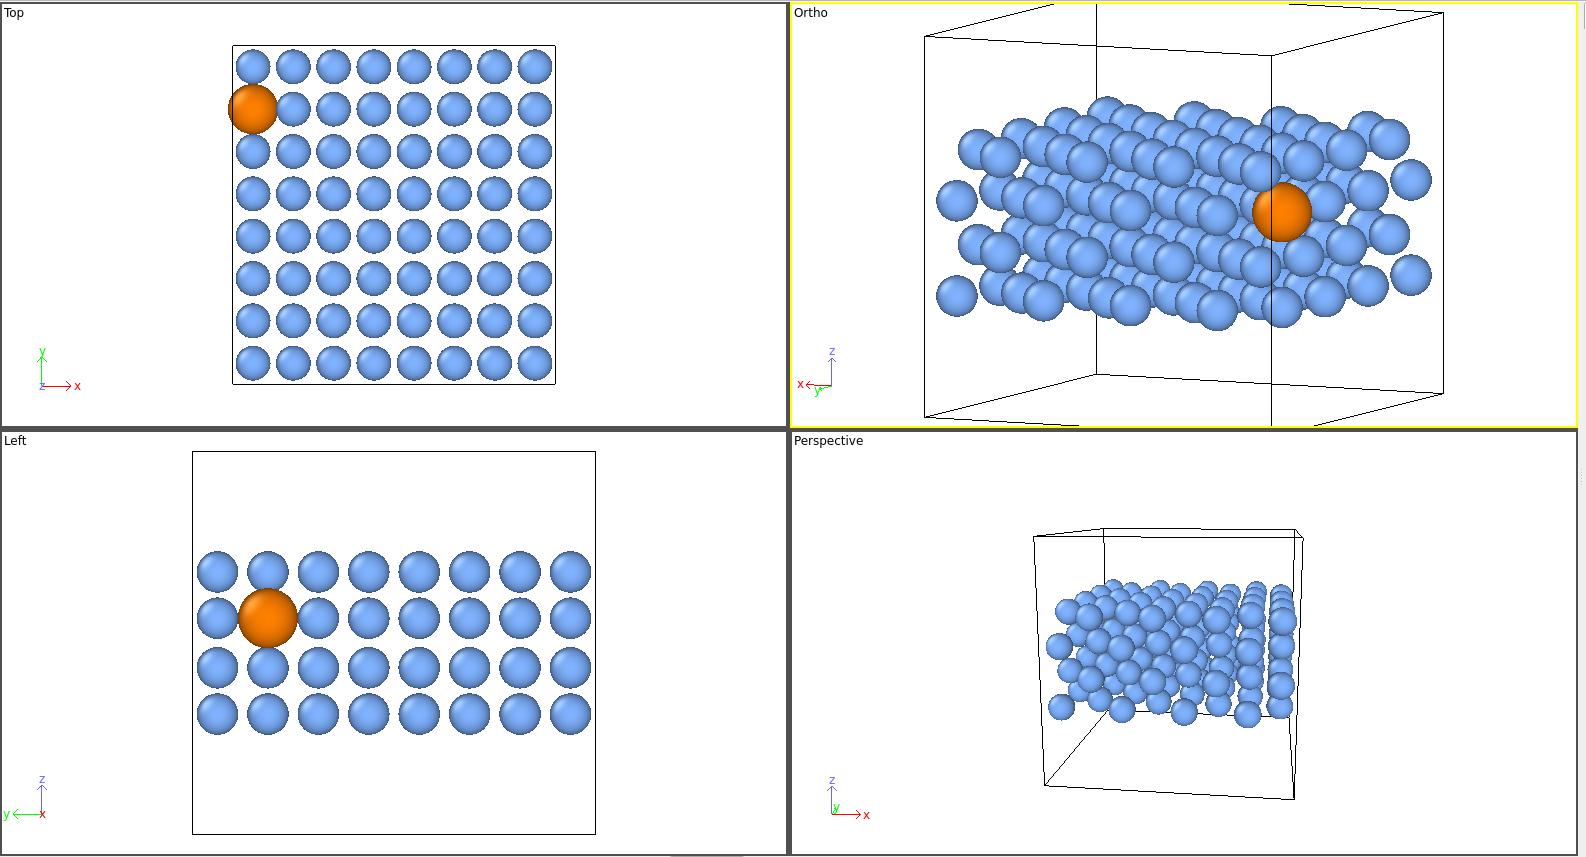
\includegraphics[width=.85\linewidth]{appendix/fepd_feru_configurations/fepd/fepdslab1.png}   
\caption{FePd Structure 04}
\label{fig:fepd04}
\end{figure}

\begin{figure}[htb]
\centering
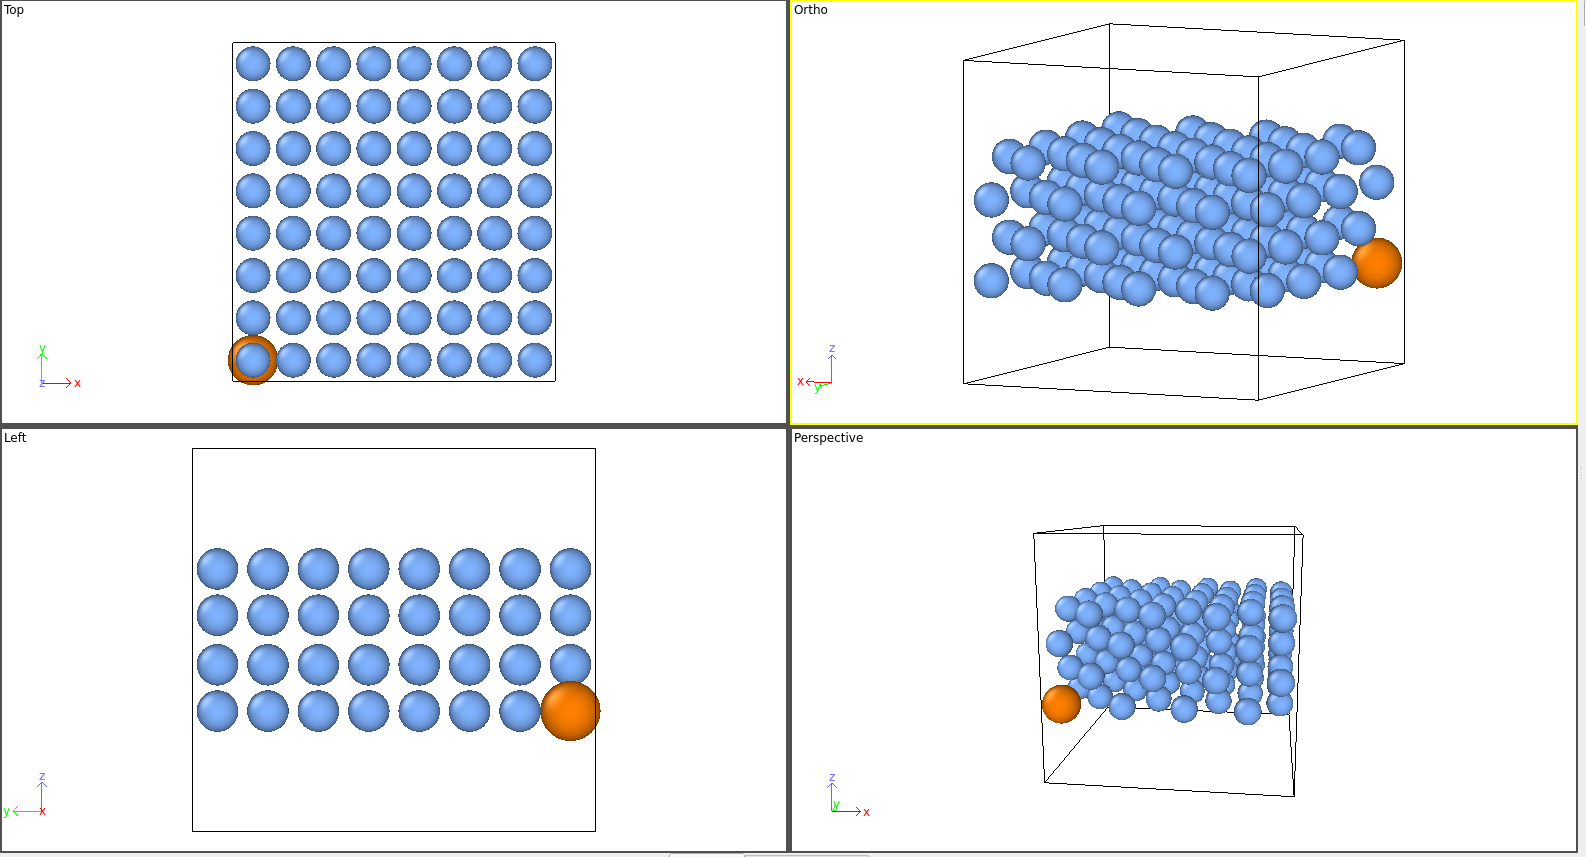
\includegraphics[width=.85\linewidth]{appendix/fepd_feru_configurations/fepd/fepdslab2.png}   
\caption{FePd Structure 05}
\label{fig:fepd05}
\end{figure}









